%% Adaptado de 
%% http://www.ctan.org/tex-archive/macros/latex/contrib/IEEEtran/
%% Traduzido para o congresso de IC da USP
%%*****************************************************************************
% Não modificar

\documentclass[twoside,conference,a4paper]{IEEEtran}

%******************************************************************************
% Não modificar
\usepackage{IEEEtsup} % Definições complementares e modificações.
\usepackage[latin1]{inputenc} % Disponibiliza acentos.
\usepackage[english,brazil]{babel}
%% Disponibiliza Inglês e Português do Brasil.
\usepackage{latexsym,amsfonts,amssymb} % Disponibiliza fontes adicionais.
\usepackage{theorem} 
\usepackage[cmex10]{amsmath} % Pacote matemático básico 
\usepackage{url} 
%\usepackage[portuges,brazil,english]{babel}
\usepackage{graphicx}
\usepackage{amsmath}
\usepackage{nccmath}
\usepackage{amssymb}
\usepackage{color}
\usepackage{ifluatex}
\usepackage[pagebackref=true,breaklinks=true,letterpaper=true,colorlinks,bookmarks=false]{hyperref}
\usepackage[tight,footnotesize]{subfigure} 
\usepackage[noadjust]{cite} % Disponibiliza melhorias em citações.
%%*****************************************************************************

\begin{document}
\selectlanguage{brazil}
\renewcommand{\IEEEkeywordsname}{Palavras-chave}

%%*****************************************************************************

\urlstyle{tt}
% Indicar o nome do autor e o curso/nível (grad-mestrado-doutorado-especial)
\title{Previsão do sucesso de chamadas de telemarketing sobre vendas de depósito bancário a longo prazo}
\author{%
 \IEEEauthorblockN{E. S. Ito\,\IEEEauthorrefmark{1}}
 \IEEEauthorblockA{\IEEEauthorrefmark{1}%
                   Ciência da Computação - Mestrado \\
                   E-mail: e159086@dac.unicamp.br}
               
 \IEEEauthorblockN{T. E. Nazatto\,\IEEEauthorrefmark{2}}
 \IEEEauthorblockA{\IEEEauthorrefmark{2}%
	Ciência da Computação - Mestrado \\
	E-mail: t074388@dac.unicamp.br}
}

%%*****************************************************************************

\maketitle

%%*****************************************************************************
% Resumo do trabalho
\begin{abstract}
Aqui avaliamos a eficiência da promoção de vendas de depósitos bancários a longo prazo para um banco português por meio de chamadas de telemarketing. Os dados utilizados foram doados e agora publicamente disponíveis para pesquisa no sítio UCI Machine Learning Repository \cite{UCI:2014}. Os dados possuem 20 variáveis (features) que potencialmente poderiam influenciar a subscrição do cliente ao programa de depósito bancário. Os mesmos serão utilizados submetidos às fases da abordagem do aprendizado de máquina: extração dos dados, preparação dos dados, seleção de features, treinamento dos dados utilizando Regressão Logística. Esses 3 modelos foram treinados com uma amostra com 90\% dos dados e treinado com uma amostra de teste com 10\% dos dados, disponibilizados pela UCI. A acurácia para os 3 modelos foram de 85\% (???). Apenas 7\% (foram influenciados pela promoção (???)
\end{abstract}

% Indique três palavras-chave que descrevem o trabalho
\begin{IEEEkeywords}
 Machine Learning (ML), dataset (DS), Regressão Logística (RL).
\end{IEEEkeywords}

%%*****************************************************************************
% Modifique as seções de acordo com o seu projeto

\section{Introdução}

Regressão Logística em Machine Learning é uma técnica de aprendizado supervisionado que consiste na regressão de um modelo matemático que relaciona variáveis de entrada $X{_i} (i=1,2,...,n)$ a diferentes grupos de classificação. Para isso, é usada a função \textit{Sigmoid} para determinar a probabilidade de um determinado conjunto de variáveis a pertencerem a determinado grupo:

\begin{ceqn}
\begin{align}
h_{\theta}(x) = \frac{1}{1+e^{-\theta^{T}x}}
\end{align}
\end{ceqn}

Como já visto anteriormente em Regressões Lineares, na Regressão Logística o melhor modelo de classificação é encontrado através da utilização do algoritmo de Gradiente Descendente, atualizando os valores de $\theta{_j}$ até encontrar o minímo da função custo $J$:
	
\begin{ceqn}
\begin{align}
J(\theta) = -\frac{1}{m}\displaystyle\sum_{i=1}^{m}y^{(i)}log(h_{\theta}(x^{(i)})) + (1-y^{(i)})log(1-h_{\theta}(x^{(i)}))
\end{align}
\end{ceqn}

Quando o melhor modelo de classificação é encontrado, tal classificação está relacionado apenas a uma classe, sendo considerado um modelo de classificação binária por apenas determinar se um dado pode ser considerado da classe em questão ou não.

A escolha do tema de eficiência da campanha de vendas de depósitos bancários a termo foi baseado no artigo de Moro et al \cite{Moro:2014} e da disponibilidade dos dados no Repositório de Dados de Machine Learning da UCI \cite{UCI:2014}. O artigo refere-se à campanha de um banco português para obter mais clientes para um produto oferecido sobre depósitos bancários a termo, uma espécie de CDB do Brasil, cuja taxa de juro é baseada no euribor3m, que é uma taxa interbancária entre bancos da União Européia, com duração de 3 meses. A campanha foi realizada por meio de chamadas telefônicas ao telefone fixo residencial ou ao celular do potencial cliente. Uma abordagem ao cliente é realizada com uma certa duração onde são explicado o produto de venda em questão e anotados uma série de dados do perfil do cliente e também do momento sócio econômico. Alguns aceitam a subscrição bancária em troca do pagamento do juros após 3 meses, baseado na taxa euribor3m, outros simplesmente não aceitam. 

Assim o banco gostaria de saber o que influencia o cliente na subscrição ao produto de venda em questão, se há possibilidade de predição de subscrição ao produto e quais dados do perfil do cliente ou quais dados do momento sócio econômico influenciam essa predição, porque se o custo-benefício de contratar uma empresa de telemarketing não compensar, poderia simplesmente diminuir o gasto com propaganda de acordo com Moro et al. \cite{Moro:2014}.

O artigo de Moro et al \cite{Moro:2014} e a disponibilidade pública do dataset na UCI \cite{UCI:2014}, também encontrado no sítio kaggle.com, junto com conteúdo dado nas aulas de Inteligência Artificial (MO416A), nos encorajaram a exercitar o tópico de machine learning.

Nos dados disponibilizados no sítio da UCI \cite{UCI:2014}, observou-se que se tratava de uma caso típico de aprendizado supervisionado, onde a variável dependente é simplesmente aceitação ou não da subscrição bancária e os dados independentes eram valores categóricos (e.g. profissão, estado conjugal, educação, etc.) e dados numéricos (e.g. idade, número de contatos, valor do euribor3m, etc.).

Dois artigos, em especial, nos serviram de guia para a elaboração deste artigo. O primeiro foi um artigo da Susan Li \cite{TowardsDataScience:2017} que descreve como a preparação dos dataset de treinamento deve ser feito, balanceamento de amostra com a utilização da técnica SMOTE (Synthetic Minority Over-sampling Technique) onde se mostra como balancear amostras com respostas positivas à subscrição e com respostas negativas à subscrição, bem como redução de features por meio da técnica RFE (Recursive Feature Elimination), técnicas segundo as quais diminuiria casos de Falsos Positivos. E o artigo Nelson Chris \cite{Medium:2019} que utiliza um técnica de Feature Engineering, onde se cria um novo campo a partir do campo pdays para representar se ouve contato anterior ou não. Este campo tem uma valor específico 999 que é usado para quando nunca ouve um prévio contato com o cliente, e em outras vezes os valores representam dias passados desde o último contato. Ambos os artigos mostram como tratar de variáveis dummy para variáveis categóricas.

Este artigo está dividido da seguinte forma. A Seção II descreve como será abordado os problemas que queremos tratar, sobre as bibliografias utilizadas como referência. A Seção III descreve a proposição do trabalho, de como será tratado a análise dos dados e como medir o desempenho da campanha de promoção de vendas de depósitos bancários. A Seção IV será descrito os materiais e métodos utilizados para aquisição, formatação dos dados, criação e teste do modelo. A Seção V mostrará os resultados dos experimentos e uma breve discussão dos resultados da análise. A Seção VI descreverá as principais conclusões do experimento.

\section{Abordagem do Problema}

A abordagem do problema será por meio das fases do Machine Learning (ML approach), como descritos nas seguintes subseções.

\subsection{Extração dos Dados}

Os dados serão extraídos da UCI \cite{UCI:2014}, onde o ds bank-additional-full.csv contém 90\% dos dados e será utilizado na fase de treinamento dos dados. O mesmo contém 41188 linhas e 20 colunas (features). E o ds bank-additional.csv contém 10\% dos dados, com 4199 linhas e 20 features ,e será utilizado para teste do modelo. Há outros dois ds, com menos dados, que não serão utilizados para este projeto. São o bank-full.csv e bank.csv.

As variáveis dos datasets (ds) extraídos da UCI \cite{UCI:2014} são as seguintes:

\begin{itemize}
	\item Dados bancários do cliente:
	
	\begin{enumerate}
		\item {\bf age:} idade (numérico)
		\item {\bf job:} tipo de trabalho (categórico: 'admin.', 'blue-collar', 'entrepreneur','housemaid', 'management', 'retired', 'self-employed', 'services', 'student', 'technician', 'unemployed', 'unknown')

		\item {\bf marital:} estado conjugal (categórico: 'divorced', 'married', 'single', 'unknown'. Nota: 'divorced' significa divorciado ou viuvez).

		\item {\bf education:} educação (categórico: 'basic.4y', 'basic.6y', 'basic.9y', 'high.school', 'illiterate', 'professional.course', 'university.degree', 'unknown')

		\item {\bf default:} está insolvente? (categórico: 'no','yes','unknown')

		\item {\bf housing:} tem empréstimo de habitação? (categórico: 'no','yes','unknown')

		\item {\bf loan:} tem empréstimo pessoal? (categórico: 'no', 'yes', 'unknown') 
relativo ao último contato da campanha corrente.

	\item {\bf contact} tipo de contato realizado (categórico: 'cellular', 'telephone').

		\item {\bf month:} mês do ano do último contato (categórico: 'jan', 'feb', 'mar', ..., 'nov', 'dec').

		\item {\bf day\_of\_week:} dia da semana do último contato (categórico: 'mon', 'tue', 'wed', 'thu', 'fri').

		\item {\bf duration:} duração do último contato em segundos (numeric). Nota importante. Este atributo afeta altamente a variável dependente (e.g. se duration=0, então y='no'). A variável duration não é conhecida antes que a chamada seja concluída. Também, após o fim da chamada, "y" é obviamente conhecido. Dessa forma, esta variável poderia ser somente incluída para propósito de benchmark e poderia ser descartado se a intenção fosse para aplicar num modelo de predição realístico. 
	\end{enumerate}

	\item Atributos do contexto social e econômico:

	\begin{enumerate}
		\setcounter{enumi}{12}
		\item {\bf emp.var.rate}: indicador trimestral da taxa de variação do emprego (numérico).

		\item {\bf cons.price.idx:} índice de preço mensal de preço ao consumidor (numérico) - semelhante ao inpc/ipca do Brasil.

		\item {\bf cons.conf.idx:} índice de confiança do consumidor - indicador mensal (numérico) - semelhante ao ICC da FGV.

		\item {\bf euribor3m:} Taxa euribor 3 meses - indicador diário (numérico).

		\item {\bf nr.employed:} número de pessoas empregadas - indicator trimestral (numérico).
	\end{enumerate}

	\item Outros atributos:

	\begin{enumerate}
		\setcounter{enumi}{17}
		\item {\bf campaign:} número de contatos realizados durante a campanha e para este cliente (numérico, inclui o último contato).

		\item {\bf pdays:} número de dias que se passaram após o último contato com o cliente desde a última campanha (numérico; 999 significa que o cliente não foi previamente contactado).

		\item {\bf previous:} número de contatos realizados antes desta campanha e para este cliente (numérico).

		\item {\bf poutcome:} resultado da campanha de marketing prévia (categórica: 'failure', 'nonexistent', 'success')
	\end{enumerate} 

	\item Variável dependente (saída do modelo/objetivo desejado):

	\begin{enumerate}
		\setcounter{enumi}{20}
		\item {\bf y:} o cliente se subscreveu ao plano de depósito a termo (binário: 'yes', 'no').
	\end{enumerate}
\end{itemize}

\subsection{Preparação dos Dados}
O notebook Project3.ipynb \footnote{https://github.com/edbkei/MO416PROJ3/tree/master/Projeto3} dá mais detalhes de como foi realizado a preparação dos dados. 

A variável dependente y foi transformado em dados binários, em vez dos dados categóricos yes e no. Bem como feito também na variável independente contact, onde o cellular ficou 0, e o telephone ficou 1.

Foi criado uma nova variável independente pdays\_no\_contact derivado do pdays, de forma que o valor 999 ficou com o valor 1 (não houve contato) e 0 (houve contato), seguindo orientação do Nelson Chris \cite{Medium:2019}. 

Foi verificado inicialmente que houve 11.26\% de subscrição e 88.72\% de não subscrição no ds de treinamento. Se utilizado o ds de treinamento sem balanceamento, haveria o risco de o modelo fazer predição com maior número de FP. Seguindo a recomendação da Susan Li \cite{TowardsDataScience:2017} , o dataset de treinamento foi balanceado utilizando o algoritmo SMOTE (Synthetic Minority Oversampling Tecnique).

As variáveis categóricas job, marital, education, default, housing, loan, month, day\_of\_week, poutcome foram transformadas em variáveis dummy, cujos valores viraram binários por meio da rotina get\_dummies da módulo pandas. Assim como exemplo, a variável categórica marital, que tem valores married, single, unknown, viraram novas variáveis binárias marital\_married, marital\_single, marital\_married. Tanto Nelson Chris como Susan Li utilizaram a técnica de criação de variáveis dummy para variáveis categóricas.

Fizemos a separação do ds de treinamento em ds da variável independente ("y") e variáveis independentes ("X") por meio do atributo loc do módulo pandas.

Realizamos também a normalização do ds das variáveis independentes ("X") por meio do algoritmo StandardScaler do módulo sklearn.

\subsection{Seleção das Features}

Com a utilização do get\_dummies, o número de variáveis aumentou de 20 para 54 variáveis independentes. Assim, Susan Li \cite{TowardsDataScience:2017} utilizou a técnica RFE (Recursive Feature Elimination) para reduzir a quantidade de features, basicamente lista-se as variáveis independente com os seus pValue por meio do aplicativo summary2 do módulo Logit. Aquelas features que tiveram o pValue maiores que 5\% seriam retirados manual da amostra. Durante o treinamento e no cross-validation (CRV), tiveram ótimo desempenho, com accuracy maior que 90\%. Porém na utilização do modelo de Regressão Logística na amostra de teste, o resultado foi pífio. Houve aumento significativo de False Positive (FP), apenas 1 caso de True Positive (TP). Resolvemos fazer como Nelson Chris \cite{Medium:2019}, i.e. manter todas as 54 variáveis independentes.

\subsection{Treinamento dos Dados}

Os dados de treinamento foram treinado com o algoritmo LogisticRegression do módulo sklearn.linear\_model. O modelo foi obtido a partir da função fit (fitness) entre os dados de treinamento balanceados e normalizados de X e y.


\subsection{Validação do Modelo}

O modelo obtido a partir da amostra de de treinamento foi também aplicado tanto para a amostra de treinamento como para a amostra de verificação e medidos pela função score para obtenção do accuracy (acurácia) do modelo.

Foi também gerado uma matriz de confusão entre o y real e o y previsto, este foi obtido da função predict à amostra X.

A matriz de confusão mostra uma matriz de 2 x 2, onde estão registrados o número de Falsos Positivos (FP), Falsos Negativos (FN), Verdadeiros Positivos (TP) e Verdadeiros Negativos (TN). Respostas verdadeiras são TP+TN, respostas falsas são FP+FN.

\subsection{Teste do Modelo}

Aqui a amostra de teste é submetida ao mesmo modelo obtido na fase de treinamento e validada no teste de CRV (Cross-Validation). Será o obtido a matriz de confusão, medido o accuracy, precision, F1-score, AUC e também será gerado o gráfico ROC.

Será verificado o número de respostas falsas e também será analisado os componentes principais que afetaram na decisão do y=1 (aceitação da subscrição).

\section{Trabalho Proposto}
O trabalho proposto será a busca do modelo de predição de subscrição ao depósito bancário por meio do processo explicado no modelo da Figura \ref{strategy}. Basicamente, essa busca ocorrerá de forma interativa tratando o dataset da UCI \cite{UCI:2014}. A aceitação do modelo no CRV e no teste de modelo será por meio dos valores das métricas. Espera-se um desempenho superior a 90\% nas métricas de precision, AUC, F1.

\begin{figure}[htbp]
	\centerline{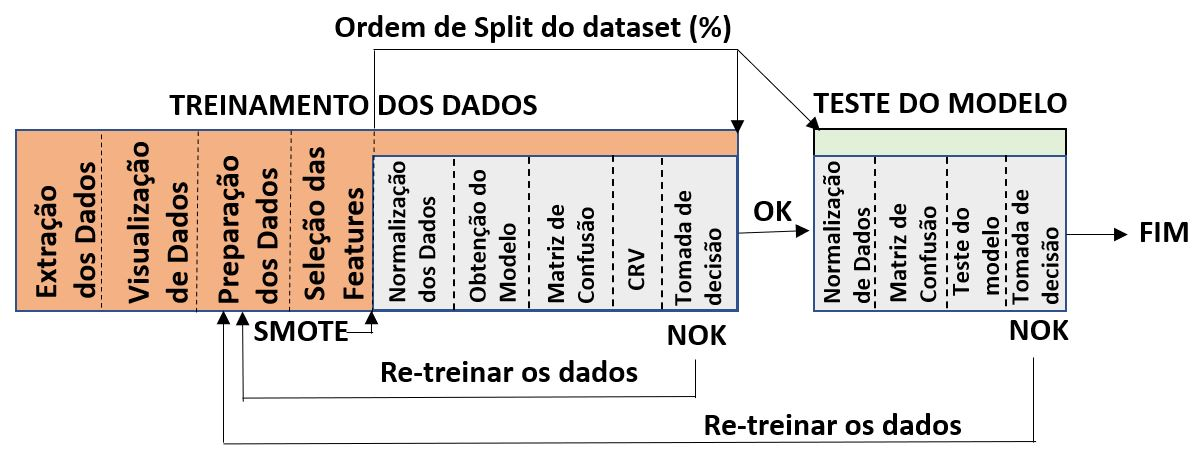
\includegraphics[scale=0.30]{figuras/strategy.jpg}}
	\caption{Estratégia de Treinamento, Cross-validation e Teste.}
	\label{strategy}
\end{figure}


\subsection{Tabelas}
Aqui a amostra de teste é submetida ao mesmo modelo obtido na fase de treinamento e validada no teste de CRV (Cross-Validation). Será o obtido a matriz de confusão, medido o accuracy, precision, F1-score, AUC e também será gerado o gráfico ROC.

Será verificado o número de respostas falsas e também será analisado os componentes principais que afetaram na decisão do y=1 (aceitação da subscrição).
A tabela \ref{tab:desempenho} contém os valores das métricas obtidas durante o CRV e teste do modelo.
%
\begin{center}
	\begin{table}[!ht]
		\caption{Tabela de Desempenho.}\label{tab:desempenho}
		\resizebox{}\textwidth}{!}{%}
		\centering    %% not "\center{...}"
		\begin{tabular}{|c|c|c|c|c|c|c|}
			\hline
			Modelo&Amostra&Score&AUC&Accuracy&Precision&F1-score\\     %% no "&" at start of row
			\hline
			LR(CRV)&70/30&0.95&0.95&0.95&0.95&0.95\\     %% no "&" at start of row
			\hline        %% extra \hline at bottom of table
			LR(Teste)&70/30&0.95&0.95&0.95&0.95&0.95\\     %% no "&" at start of row
			\hline        %% extra \hline at bottom of table
	\end{tabular}}
\end{table}
\end{center}


\section{Materiais e Métodos}

Todo trabalho deve ser submetido a algum tipo de teste para que possa ser avaliado. Na verdade, buscamos aqui uma validação com um caráter mais científico de seu trabalho (validação de hipótese). Busca-se identificar quais os seus pontos fortes e fracos. Nesta seção você deve descrever claramente quais foram e como foram conduzidos os testes, quais os materiais e as metodologias empregadas.   

Uma figura pode ser posicionada em qualquer lugar no texto, como no exemplo seguinte da Figura~\ref{fig:fig1}.

Use o comando ``cite'' para citar itens na sua lista de
referências através dos seus rótulos. Exemplo: \cite{Moro:2014}\cite{UCI:2014}.


\section{Resultados e Discussão}

Nesta seção você deve apresentar claramente os resultados obtidos para os testes efetuados. Procure organizar os dados utilizando uma linguagem científica. Algumas opções são o uso de tabelas e gráficos, para que a compreensão seja fácil e rápida. 

\section{Conclusões}

Nesta seção, faça uma análise geral de seu trabalho, levando em conta todo o processo de desenvolvimento e os resultados. Quais os seus pontos fortes? Quais os seus pontos fracos? Quais aspectos de sua metodologia de trabalho foram positivas? Quais foram negativas? O que você recomendaria (ou não recomendaria) a outras pessoas que estejam realizando trabalhos similares aos seus? 

A campanha de promoção de vendas de depósito bancário à prazo, por meio de telemarketing, obteve subscrição de apenas 11 \% dos potenciais clientes abordados. Possivelmente, devido ao fato que a abordagem para determinadas classes ou condições sociais econômicas sejam impeditivas ou não entenderem o tipo de investimento que lhes são propostos. Depósito bancário à prazo pode ser interessante se os juros pagos no resgate forem também interessantes. O euribor3m é a é taxa interbancária contra a qual um grupo representativo de bancos europeus contrai empréstimos mutuamente cuja duração é de 3 meses, muito similar o CDB do Brasil, o ajuste de juros de empréstimos, conta poupança, hipoteca, etc seguem essa taxa. O nosso modelo indicou o eurobor3m como feature importante, como esperado que fosse. Algumas pessoas veem valor com esse tipo de transação bancária, pois pode emprestar o dinheiro por um tempo para o banco em troca de juros, como é o caso de aposentados (job\_retired) e estudantes (job\_student), pois tem nível universitário (education\_university.degree) e portanto é de se esperar que entendam o mecanismo da aplicação financeira. O clima econômico parece favorecer potenciais clientes para aquisição da aplicação como indica a média trimestral do número total de cidadãos empregados (nr.employed) e a taxa de variação de empregabilidade trimestral (emp.var.rate). A enquete durante a campanha mostra que potenciais clientes escondem se os mesmos tem algum problema com débitos pendentes (default\_unknown). Contato por meio de telefone ou celular (contact), ou mais de um contato (campaign), com o cliente, também se já houve um contato prévio bem sucedido (poutcome\_success) ou não existente (poutcome\_nonexistent), com uma certa duração (duration), parecem influir na aquisição do plano do depósito à prazo. Alguns meses no ano tiveram melhor aceitação da campanha como março, maio, julho, agosto, setembro, novembro e dezembro. O melhor dia da semana para abordar clientes foi quarta-feira.

%******************************************************************************
% Referências - Definidas no arquivo Relatorio.bib
 +-------------+

\bibliographystyle{IEEEtran}

\bibliography{Relatorio}


%******************************************************************************

\vspace{20ex}

\section*{\Large \textbf{Submissão}}

Seu trabalho deve ser submetido via Google ClassRoom.

\vspace{3ex}

\begin{center}
 {\Large \textbf{\textsc{Prazo: 09/08/2020}}}
\end{center}

\end{document}
